\documentclass{slide}
\usepackage{tikz}
\usetikzlibrary{snakes}
\usetikzlibrary{intersections}
\usetikzlibrary{shapes.geometric}

\usepackage{languages}

\title{Development Tips}
\subtitle{CSSE6400}
\author{Brae Webb}
\date{\week{11}}

\begin{document}

\maketitle

\questionanswer{What did we \highlight{learn} from the cloud assignment?}{Cloud development is \highlight{painful}?}

\question{How can we make this \highlight{less} painful?}

\point[Some ideas]{
\begin{enumerate}
    \item Gain confidence through \highlight{testing}
    \item \highlight{Automate} what you're repeating
    \item \highlight{Tighten feedback loop} as much as possible
    \item \highlight{Log and monitor} what you can
\end{enumerate}
}

\point{
    Gain confidence through \highlight{testing}
}

\point[The testing elephant in the room]{Test-driven development}

\point[TDD in theory]{
    \begin{center}
    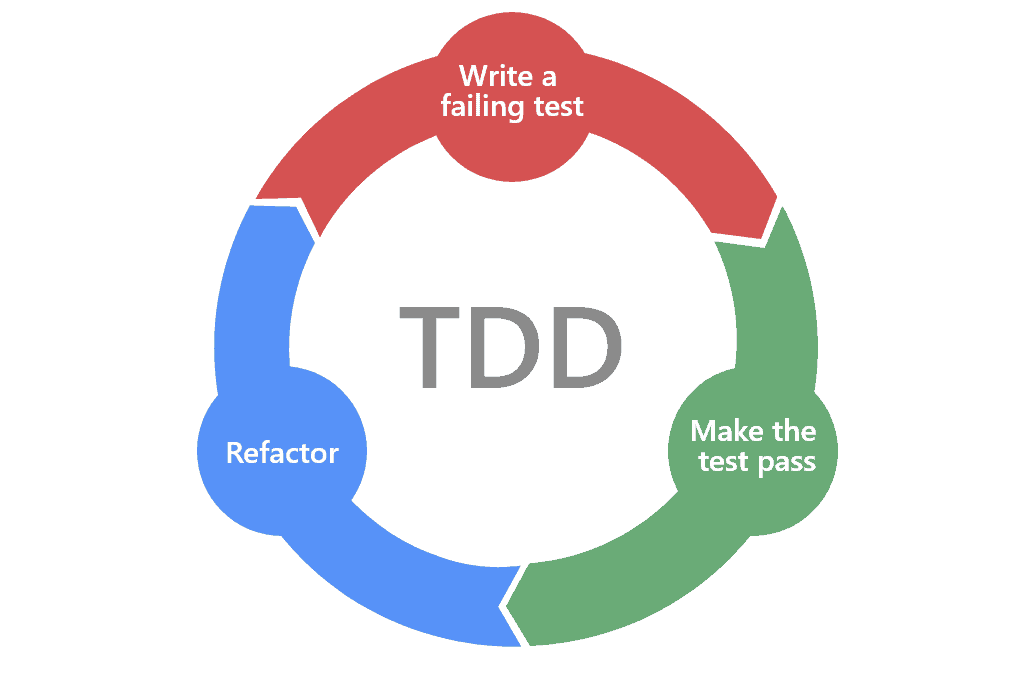
\includegraphics[width=0.6\textwidth]{images/tdd}\normalsize\cite{tdd-loop}
    \end{center}
}

\point[What do you primarily get from TDD?]{
\begin{enumerate}[<+->]
    \item Regression tests (confidence)
    \item Small isolated components
\end{enumerate}
}

\questionanswer{Do you have to use TDD to get these benefits?}{No. \only<3->{But it can make it easier.}}

\questionanswer{When should you write a test?}{Whenever you are checking manually something often}

\point[Examples]{
\begin{itemize}[<+->]
    \item Checking the endpoints your API.
    \item Checking a feature in the frontend of your interface.
\end{itemize}
}


\point{
    \highlight{Automate} what you're repeating
}

\point[Examples]{
\begin{itemize}[<+->]
    \item Running tests.
    \item Starting locally and running tests locally.
    \item Deployment (\texttt{deploy.sh}).
    \item Deployment and running tests.
\end{itemize}
}

% \point{Bash is your friend.}

\point{
    \highlight{Tighten feedback loop} as much as possible
}

\point[Examples]{
\begin{itemize}[<+->]
    \item Containers
    \item Local database (docker-compose)
    \item Local cloud services (e.g. S3)
\end{itemize}
}

\point{
    \highlight{Log and monitor} what you can
}

\point{Refer to week 9 content}

\point[Tip]{Enable CloudWatch on EC2}

\point[Aside]{Environment variables}

\references{dev-tips}


\end{document}